\documentclass[tikz,border=8pt]{standalone}
\usepackage[T1]{fontenc}
\usepackage[utf8]{inputenc}
\usepackage{amsmath,amssymb}
\usetikzlibrary{arrows.meta,calc}

\begin{document}
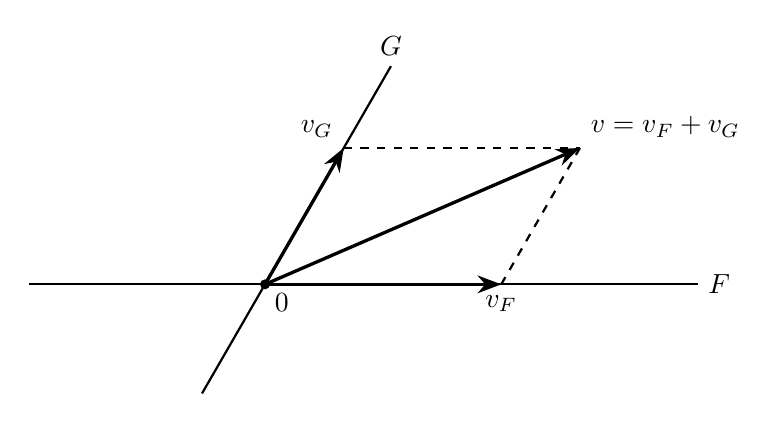
\begin{tikzpicture}[
  >={Stealth[length=3mm]},
  droite/.style={thick},
  vect/.style={very thick,->},
]
  % Coordonnees
  \coordinate (O)  at (0,0);
  \coordinate (vF) at (3,0);    % composante suivant F
  \coordinate (vG) at (60:2);   % composante suivant G
  \coordinate (v)  at ($(vF)+(vG)$);

  % Sous-espaces F et G (droites vectorielles)
  \draw[droite] (-3,0) -- (5.5,0) node[right] {$F$};
  \draw[droite] (60:-1.6) -- (60:3.2) node[above] {$G$};

  % Parallelogramme (traits pointilles)
  \draw[dashed,thick] (vG) -- (v);
  \draw[dashed,thick] (vF) -- (v);

  % Vecteurs
  \draw[vect] (O) -- (vF) node[below] {$v_F$};
  \draw[vect] (O) -- (vG) node[above left] {$v_G$};
  \draw[vect] (O) -- (v)  node[above right] {$v = v_F + v_G$};

  % Origine
  \fill (O) circle (1.8pt) node[below right] {$0$};
\end{tikzpicture}
\end{document}

